\chapter{Appendix: Results}
In this appendix are collected all results of
\begin{itemize}
    \item feature selection evaluated by fs\_results.ipynb;
    \item model prediction errors by Keras\_prediction\_model.ipynb and RandomForest\_prediction\_model.ipynb;
\end{itemize}
\pagebreak
\clearpage
\section{Feature Selection results}
\subsection{Borda Count results}
\begin{figure}[H]
\vspace*{\fill}
\vspace{-\topskip}
\centering
\subfloat[10 Km resolution with mountains]{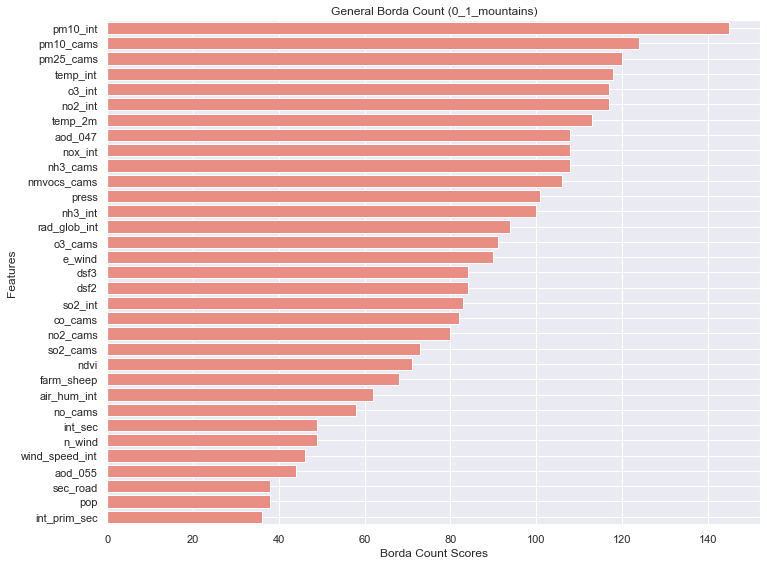
\includegraphics[scale =0.42]{images/tests/0_1_mountainspm25_st.png}}\\
\subfloat[10 Km resolution with mountains]{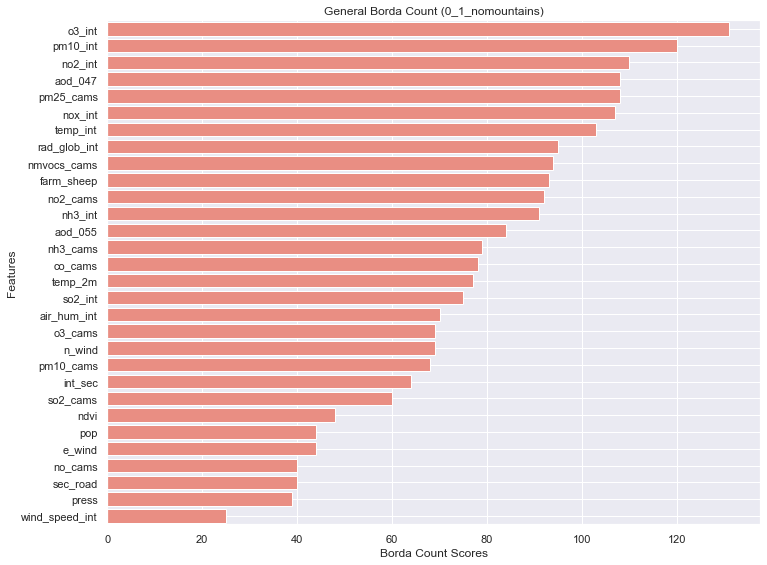
\includegraphics[scale =0.42]{images/tests/0_1_nomountainspm25_st.png}}
\caption{FS results obtained with fine particulate ('pm25\_st') as target variable and 10 km resolution.}
\vspace{\fill}

\end{figure}
\begin{figure}[H]
\centering
\subfloat[10 Km resolution with mountains]{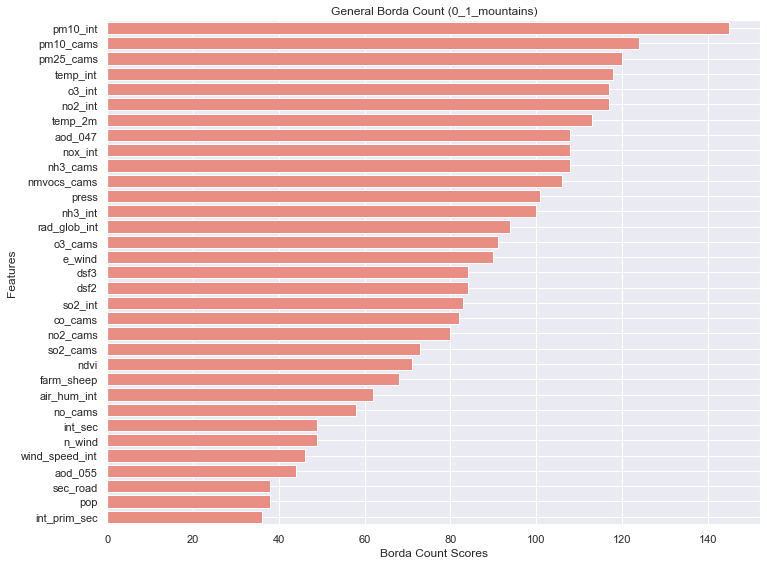
\includegraphics[scale =0.42]{images/tests/0_1_mountainspm25_st.png}}\\
\subfloat[10 Km resolution with mountains]{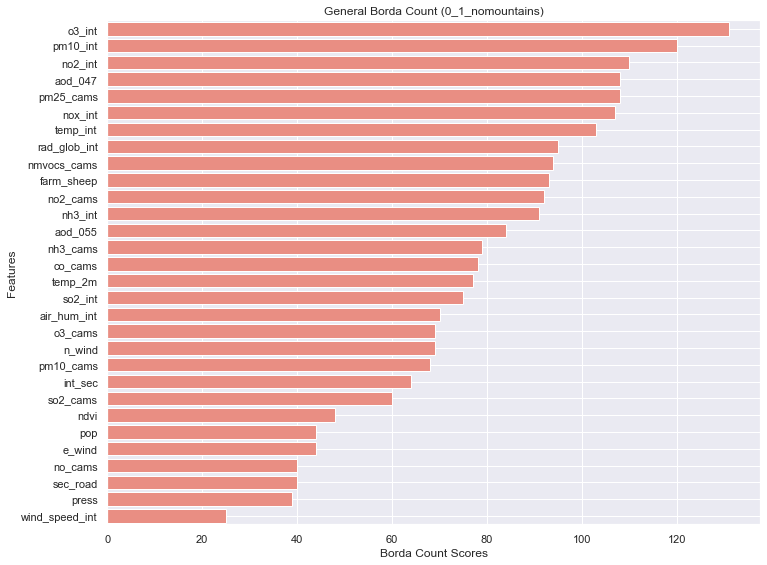
\includegraphics[scale =0.42]{images/tests/0_1_nomountainspm25_st.png}}
\caption{FS results obtained with fine particulate ('pm25\_st') as target variable and 10 km resolution.}
\end{figure}
\begin{figure}[H]
\centering
\subfloat[1 Km resolution with mountains]{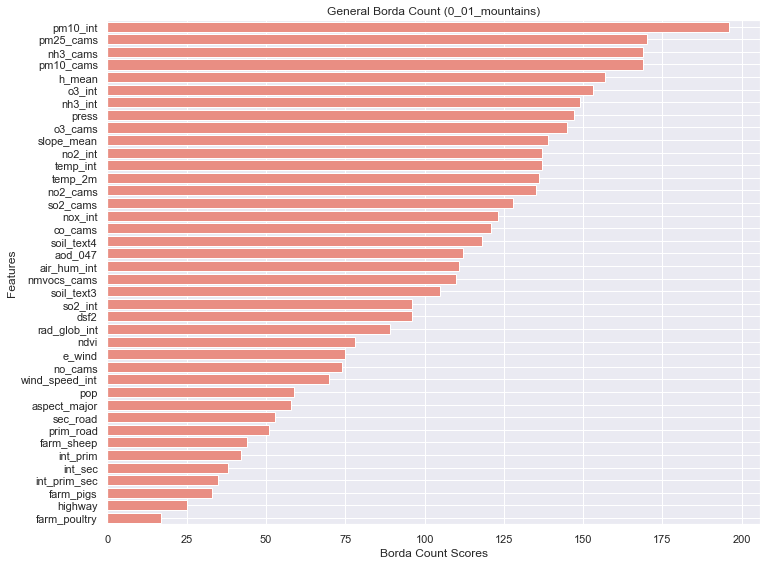
\includegraphics[scale =0.42]{images/tests/0_01_mountainspm25_st.png}}\\
\subfloat[1 Km resolution with mountains]{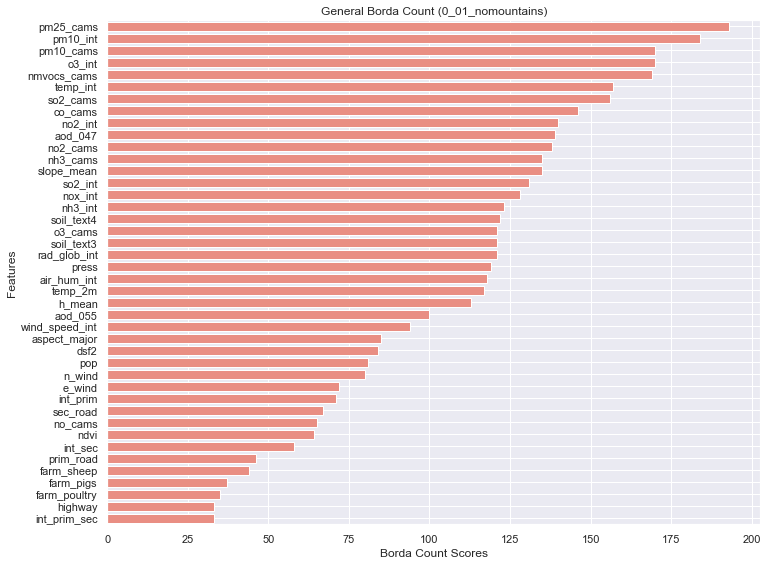
\includegraphics[scale =0.42]{images/tests/0_01_nomountainspm25_st.png}}
\caption{FS results obtained with fine particulate ('pm25\_st') as target variable and 1 km resolution.}
\end{figure}
\begin{figure}[H]
\centering
\subfloat[10 Km resolution with mountains]{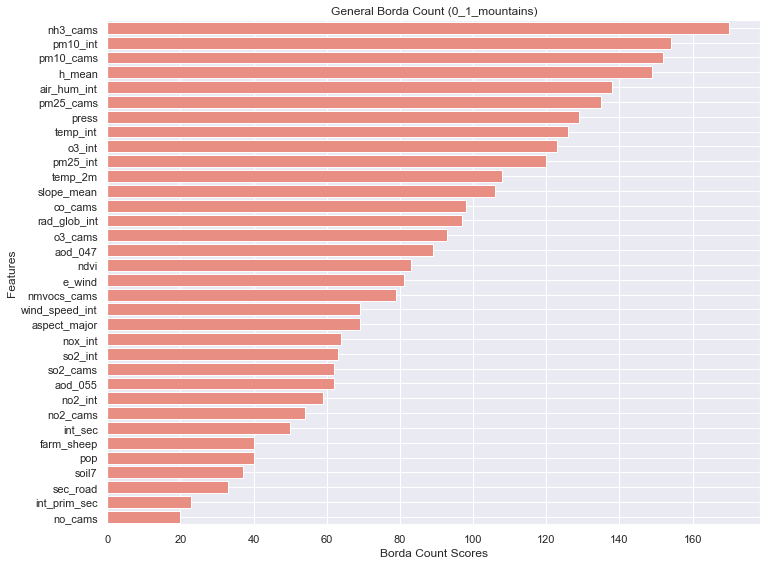
\includegraphics[scale =0.42]{images/tests/0_1_mountainsnh3_st.png}}\\
\subfloat[10 Km resolution with mountains]{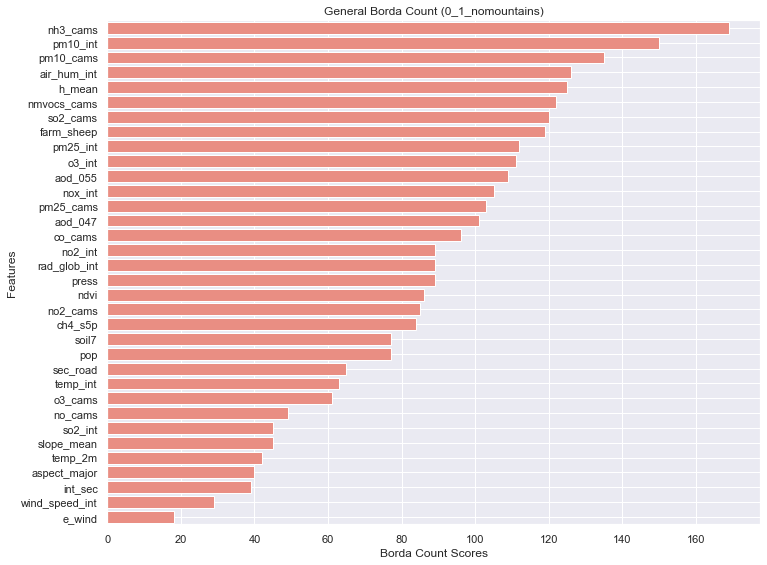
\includegraphics[scale =0.42]{images/tests/0_1_nomountainsnh3_st.png}}
\caption{FS results obtained with ammonia ('nh3\_st') as target variable and 10 km resolution.}
\end{figure}
\begin{figure}[H]
\centering
\subfloat[1 Km resolution with mountains]{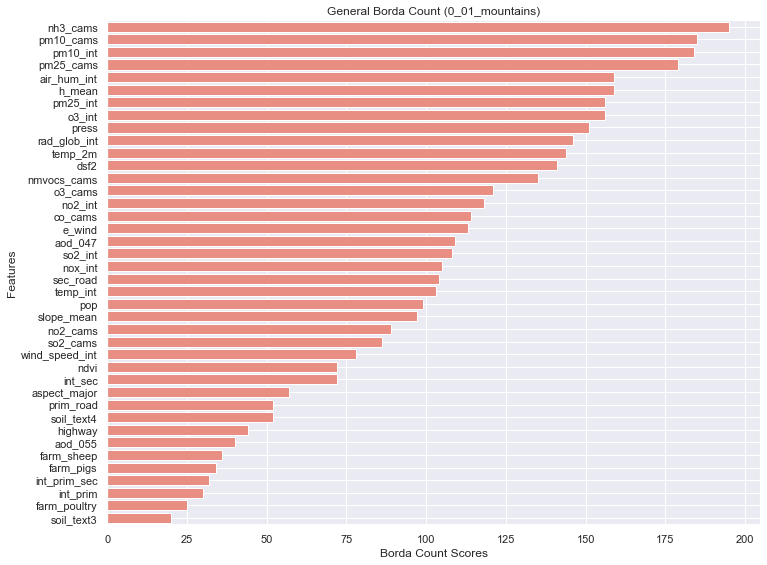
\includegraphics[scale =0.42]{images/tests/0_01_mountainsnh3_st.png}}\\
\subfloat[1 Km resolution with mountains]{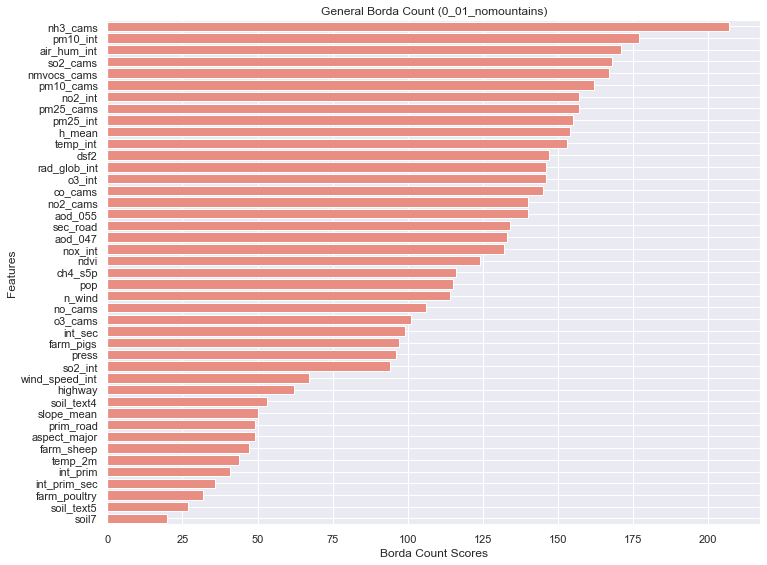
\includegraphics[scale =0.42]{images/tests/0_01_nomountainsnh3_st.png}}
\caption{FS results obtained with ammonia ('nh3\_st') as target variable and 1 km resolution.}
\end{figure}
\subsection{Pearson correlation index results}
\begin{figure}[H]
    \centering
    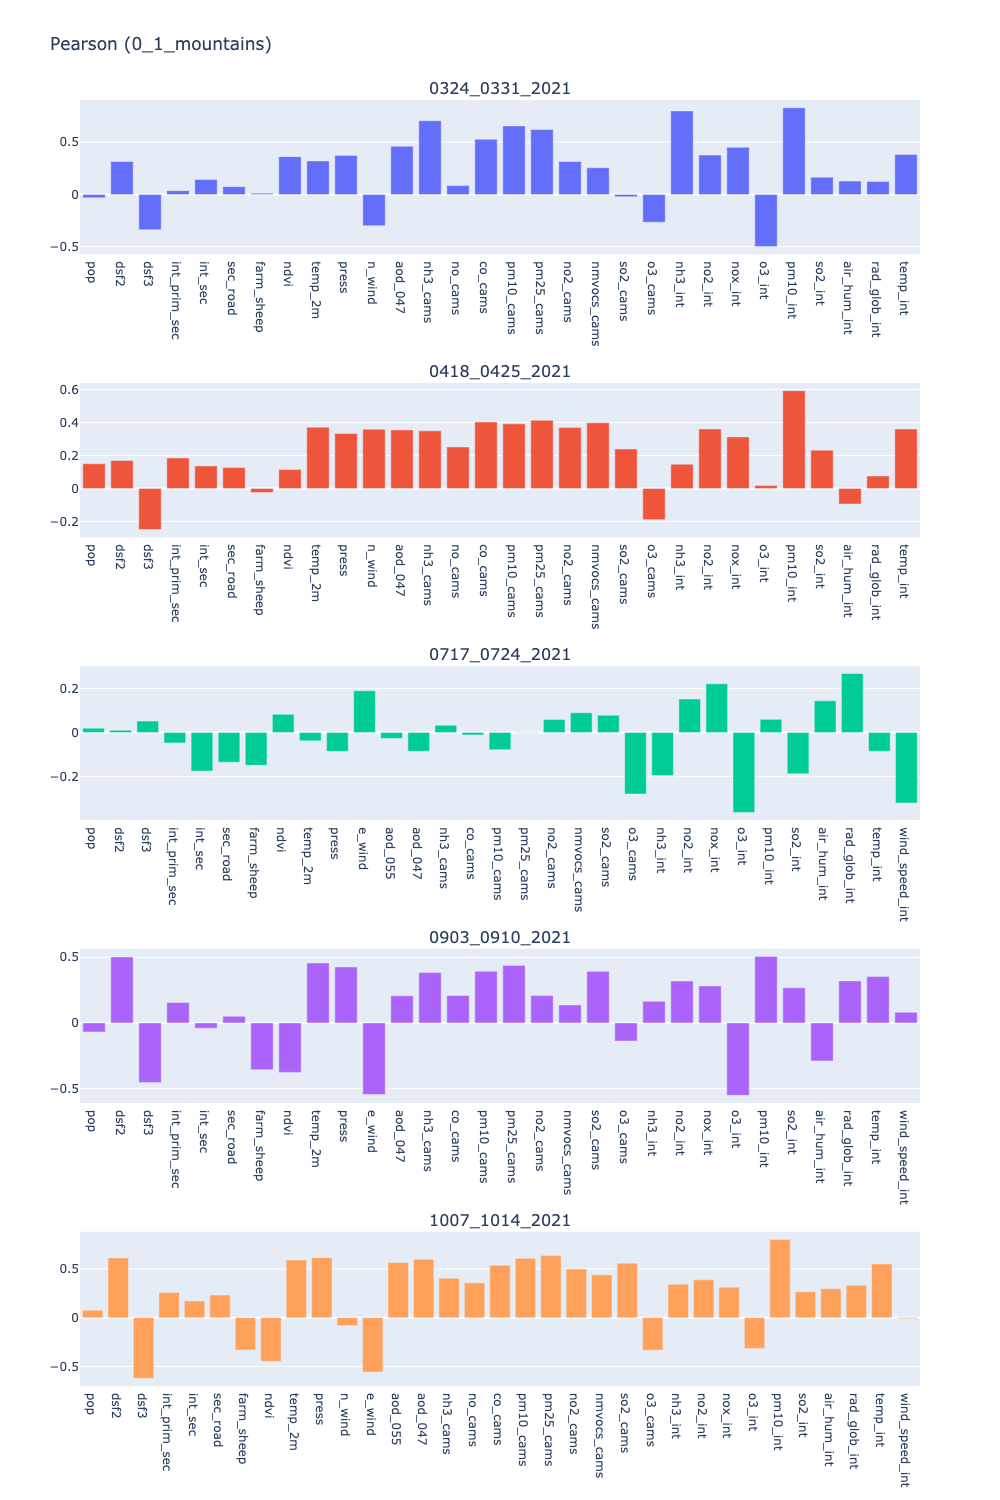
\includegraphics[scale=0.35]{images/tests/0_1_mountainspm25_st_pearson.png}
    \caption{Pearson correlation index results with respect to fine particulate ('pm25\_st') as target variable, with 10km resolution including mountains.}
\end{figure}
\begin{figure}[H]
    \centering
    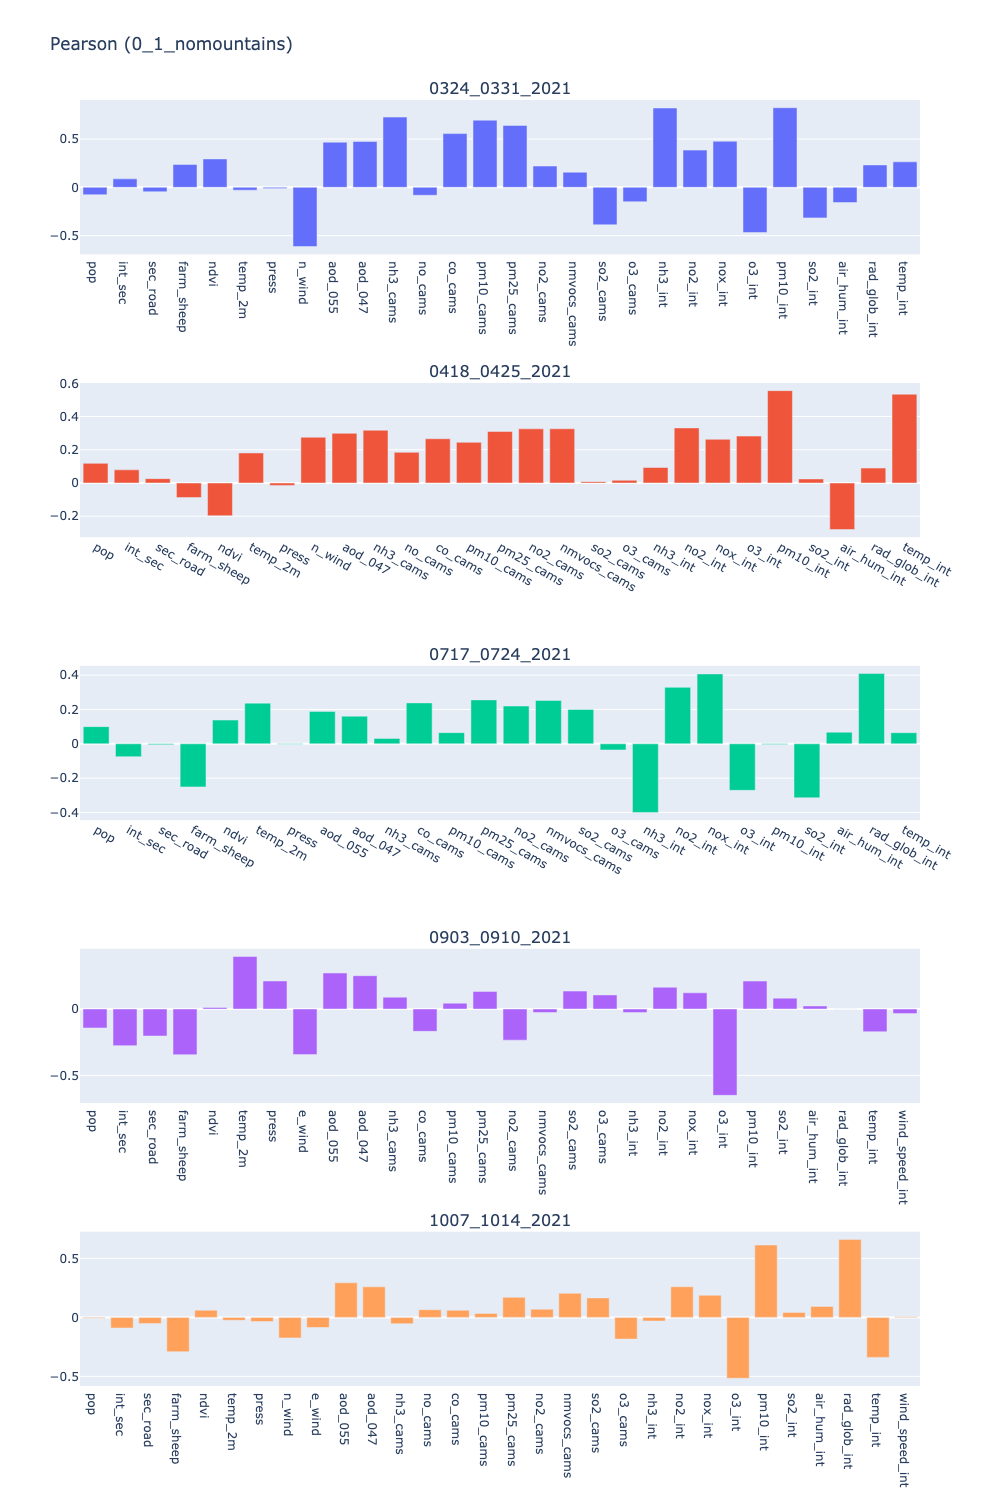
\includegraphics[scale=0.35]{images/tests/0_1_nomountainspm25_st_pearson.png}
    \caption{Pearson correlation index results with respect to fine particulate ('pm25\_st') as target variable, with 10km resolution excluding mountains.}
    
\end{figure}
\begin{figure}[H]
    \centering
    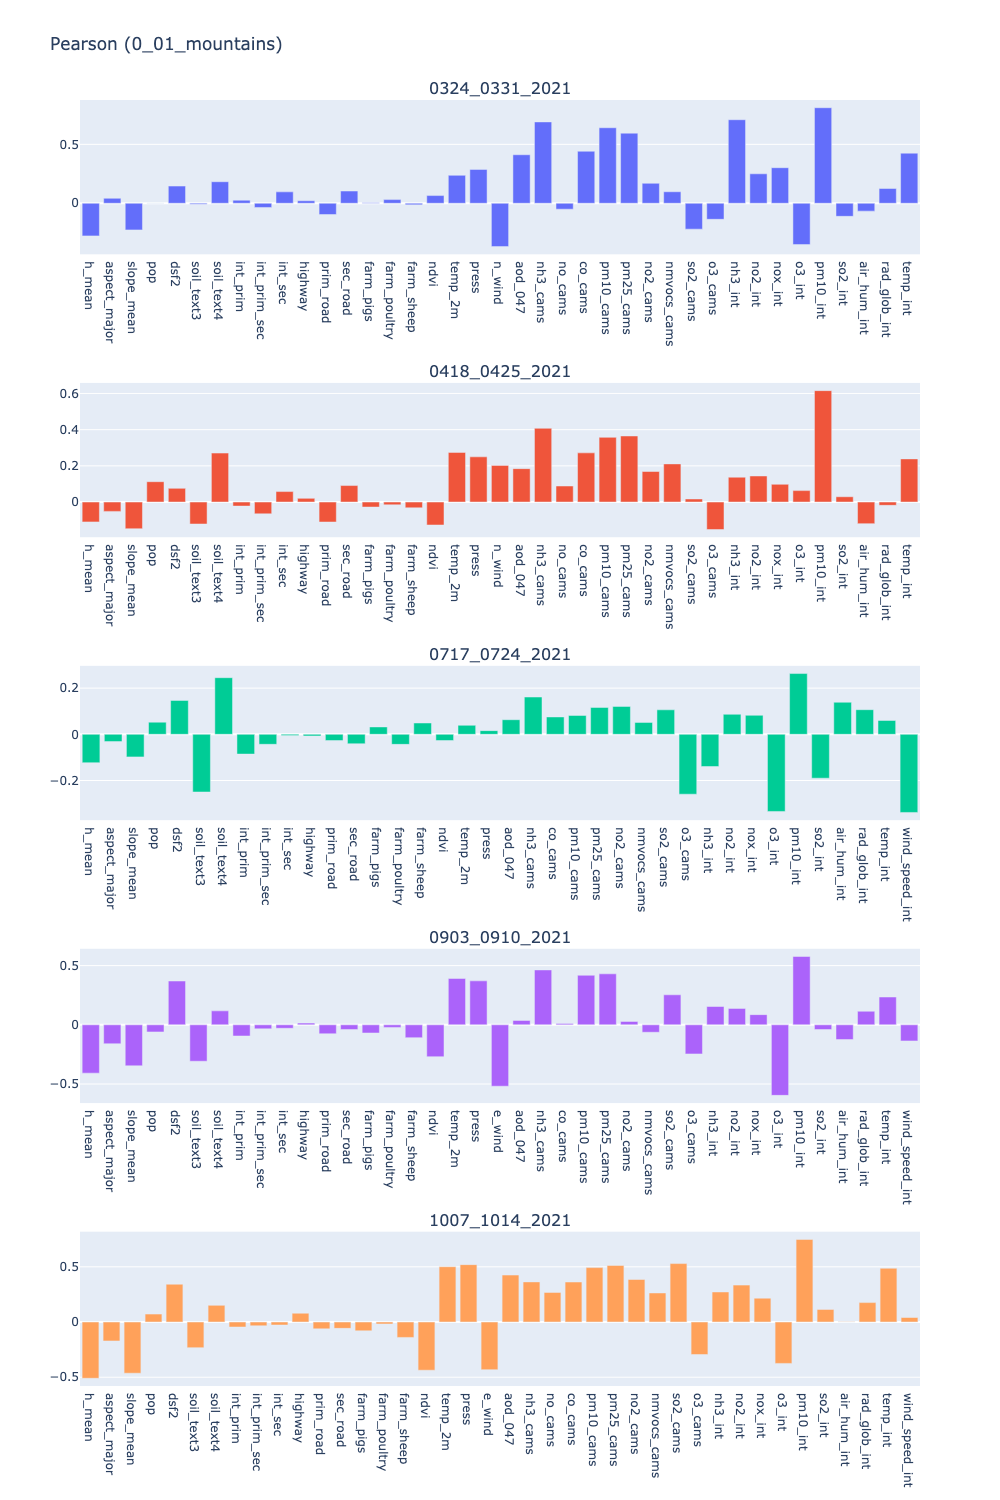
\includegraphics[scale=0.35]{images/tests/0_01_mountainspm25_st_pearson.png}
    \caption{Pearson correlation index results with respect to fine particulate ('pm25\_st') as target variable, with 1km resolution including mountains.}
    
\end{figure}
\begin{figure}[H]
    \centering
    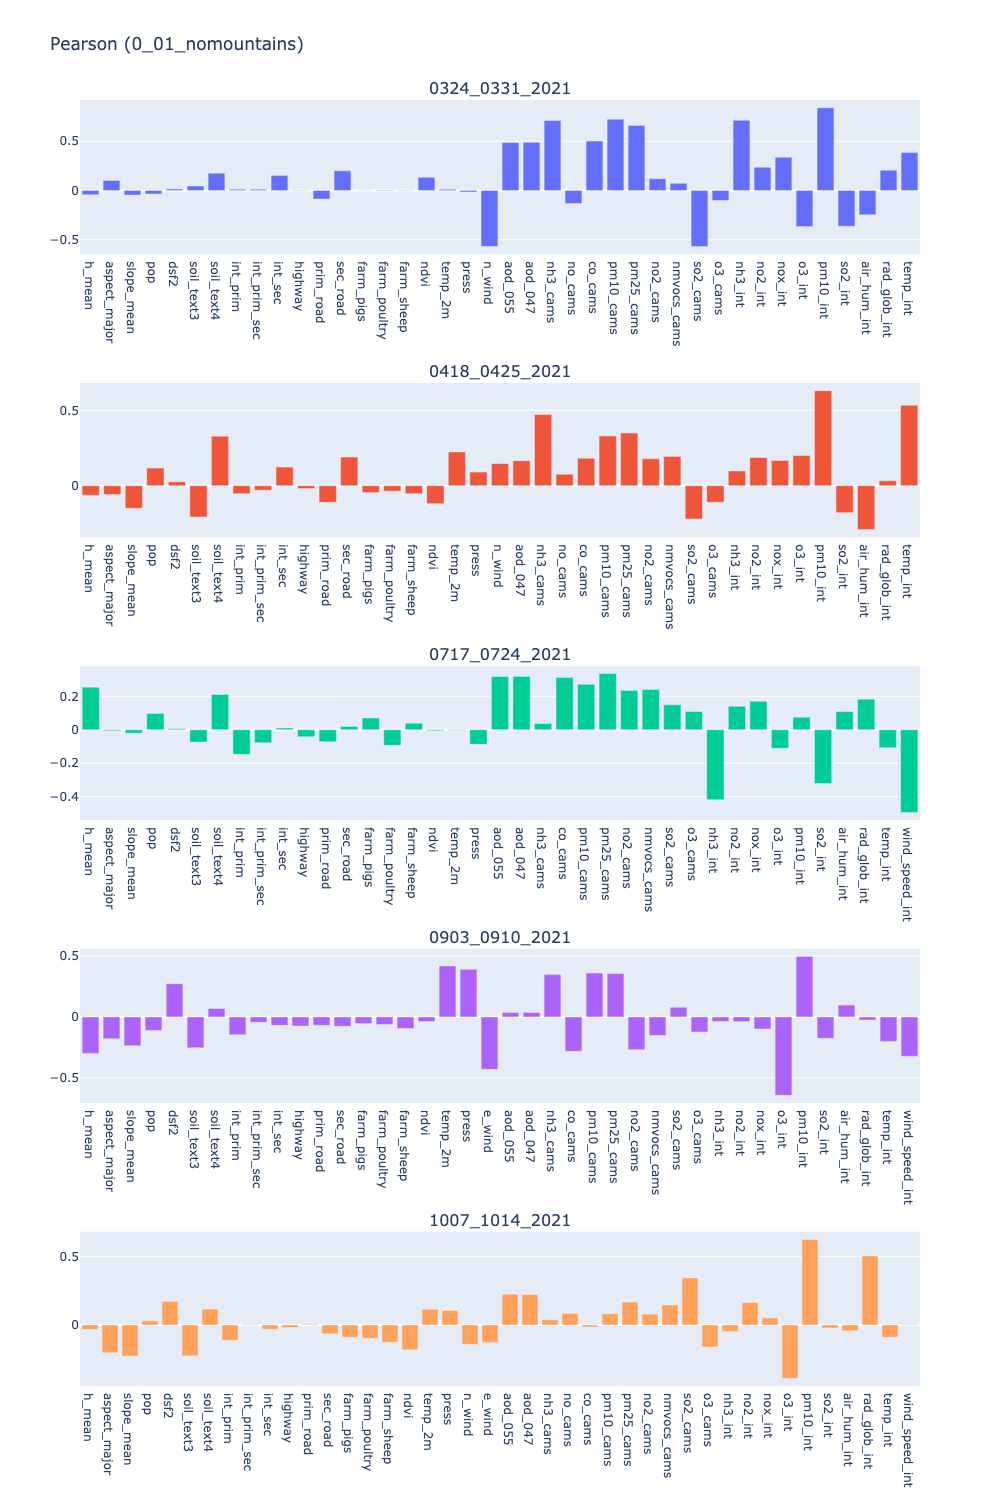
\includegraphics[scale=0.35]{images/tests/0_01_nomountainspm25_st_pearson.png}
    \caption{Pearson correlation index results with respect to fine particulate ('pm25\_st') as target variable, with 1km resolution excluding mountains.}
    
\end{figure}


\begin{figure}[H]
    \centering
    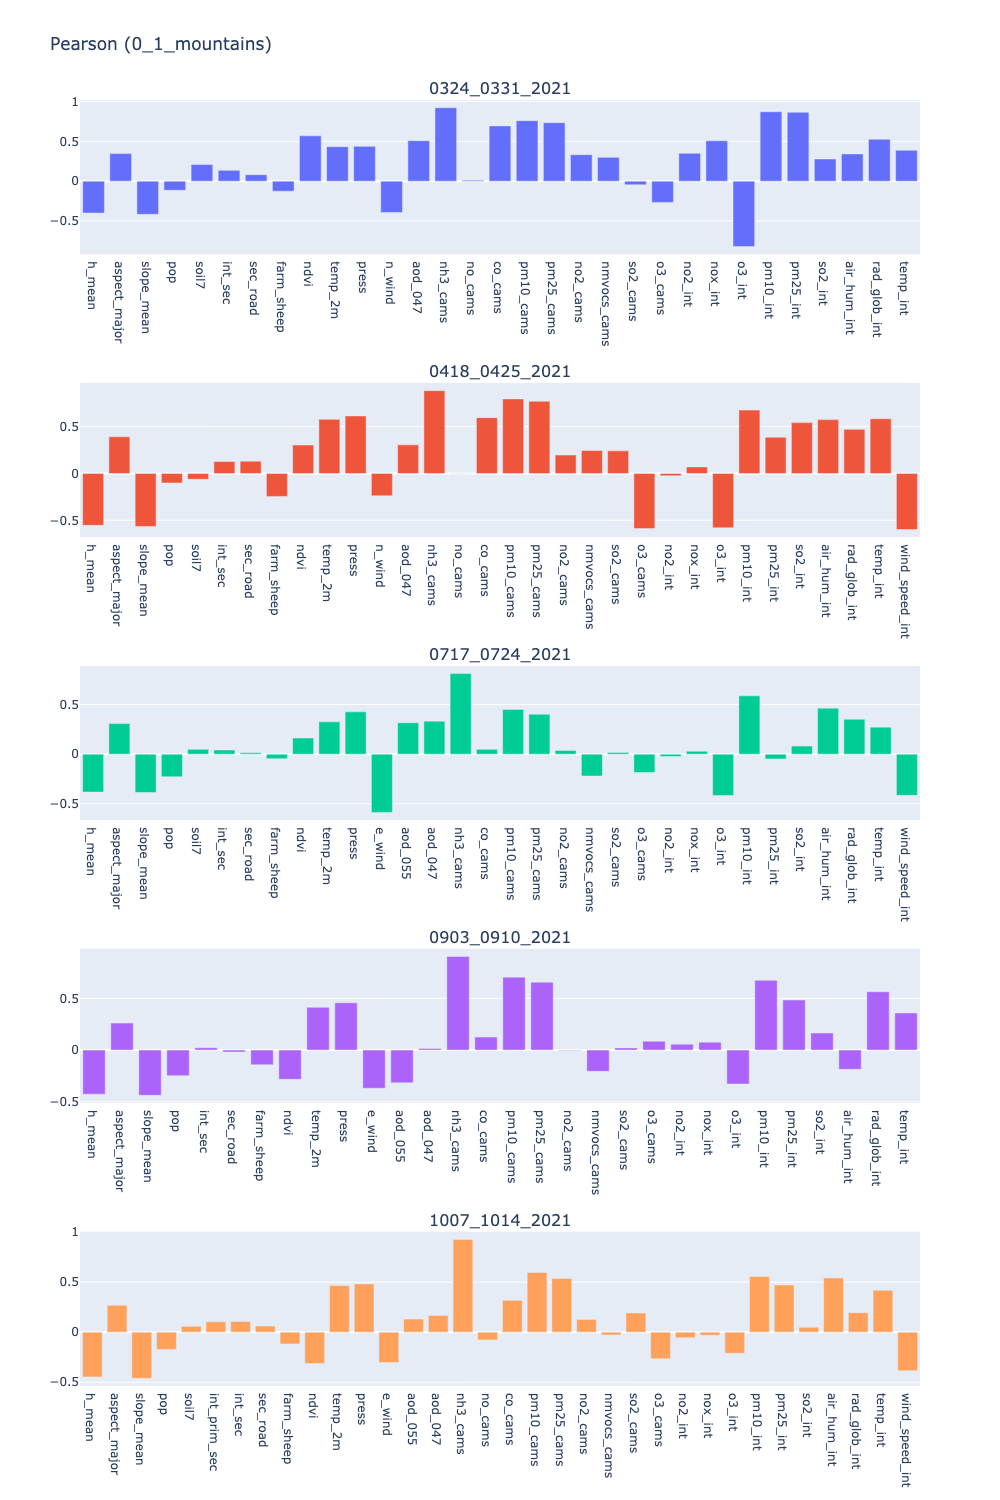
\includegraphics[scale=0.35]{images/tests/0_1_mountainsnh3_st_pearson.png}
    \caption{Pearson correlation index results with respect to ammonia ('nh3\_st') as target variable, with 10km resolution including mountains.}
    
\end{figure}
\begin{figure}[H]
    \centering
    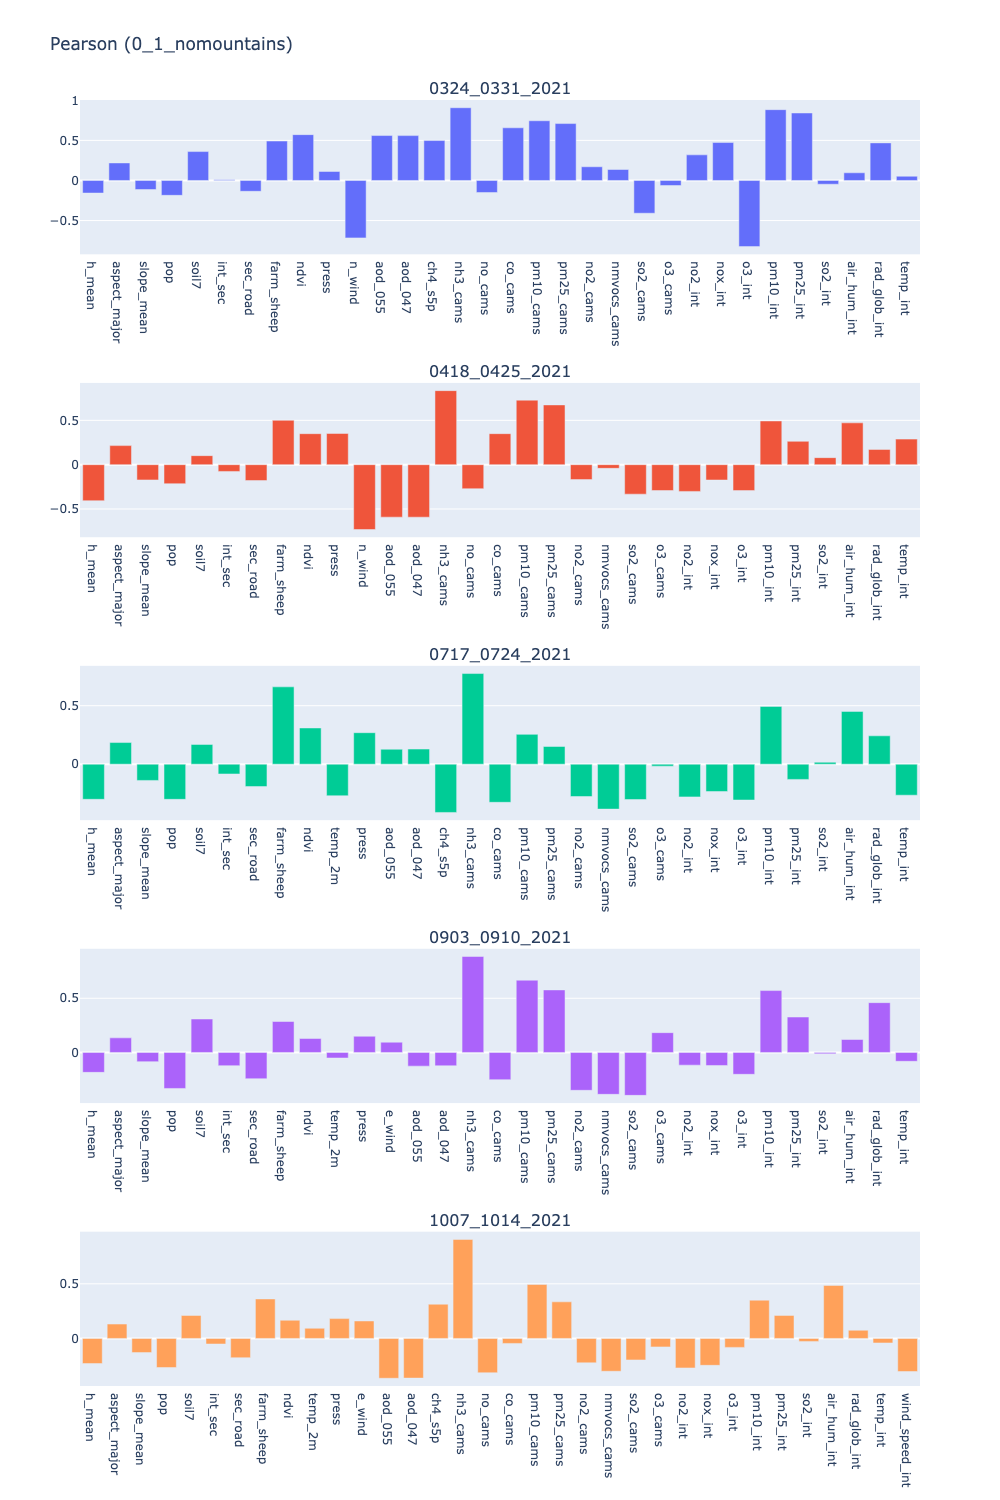
\includegraphics[scale=0.35]{images/tests/0_1_nomountainsnh3_st_pearson.png}
    \caption{Pearson correlation index results with respect to ammonia ('nh3\_st') as target variable, with 10km resolution excluding mountains.}
    
\end{figure}
\begin{figure}[H]
    \centering
    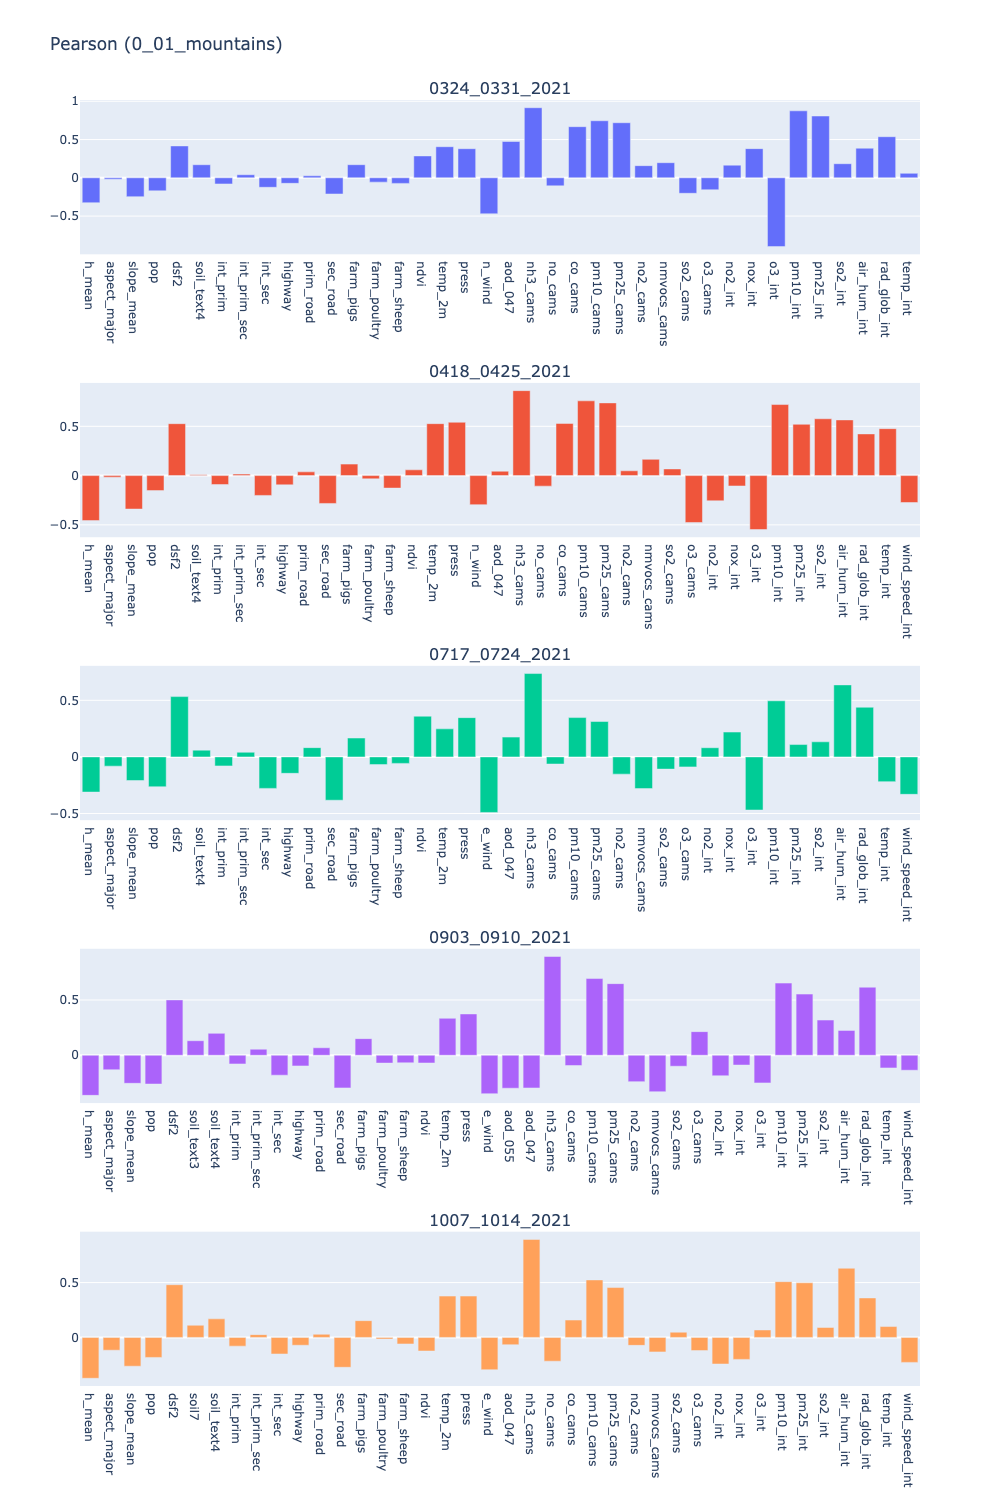
\includegraphics[scale=0.35]{images/tests/0_01_mountainsnh3_st_pearson.png}
    \caption{Pearson correlation index results with respect to ammonia ('nh3\_st') as target variable, with 1km resolution including mountains.}
    
\end{figure}
\begin{figure}[H]
    \centering
    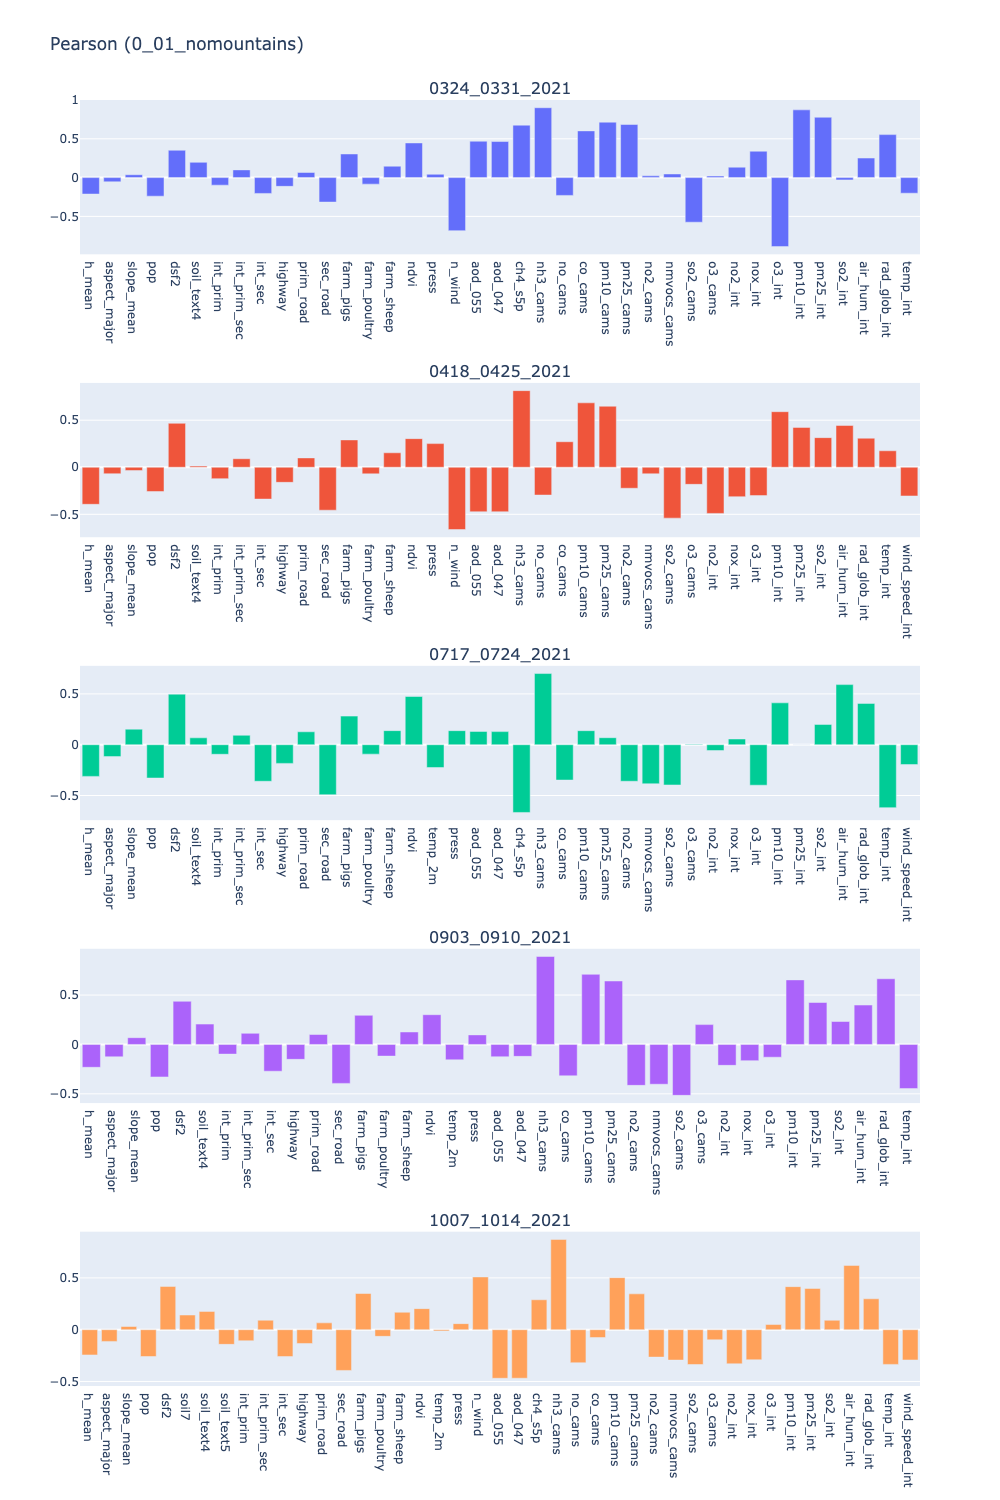
\includegraphics[scale=0.35]{images/tests/0_01_nomountainsnh3_st_pearson.png}
    \caption{Pearson correlation index results with respect to ammonia ('nh3\_st') as target variable, with 1km resolution excluding mountains.}
    
\end{figure}

\section{ML models results}
\subsection{Random Forest}

\begin{table}[H]
\begin{tabular}{lrrrrr}
\toprule
  &  24/03-31/03 &  18/04-25/04 &  17/07-24/07 &  3/09-10/09 &  7/10-14/10 \\
\midrule
 MAE\_sensor &        1.217 &        0.967 &        0.593 &       0.910 &       0.761 \\
RMSE\_sensor &        1.769 &        1.235 &        0.797 &       1.233 &       1.034 \\
 MSE\_sensor &        3.218 &        1.532 &        0.636 &       1.593 &       1.107 \\
  R2\_sensor &        0.883 &        0.778 &        0.681 &       0.852 &       0.851 \\
   MAE\_cams &        7.800 &        6.556 &        2.110 &       3.060 &       3.478 \\
  RMSE\_cams &        9.262 &        7.571 &        2.745 &       3.623 &       4.059 \\
   MSE\_cams &       86.279 &       57.593 &        7.548 &      13.266 &      16.591 \\
    R2\_cams &       -2.147 &       -7.492 &       -2.846 &      -0.258 &      -1.096 \\
\bottomrule
\end{tabular}
\caption{Random Forest prediction for PM2.5 with 10 km resolution, including zones with mountains.}
\end{table}
\bigskip
\begin{table}[H]
\begin{tabular}{lrrrrr}
\toprule
  &  24/03-31/03 &  18/04-25/04 &  17/07-24/07 &  3/09-10/09 &  7/10-14/10 \\
\midrule
 MAE\_sensor &        1.350 &        1.132 &        0.606 &       0.908 &       0.834 \\
RMSE\_sensor &        1.798 &        1.448 &        0.818 &       1.226 &       1.113 \\
 MSE\_sensor &        3.254 &        2.131 &        0.709 &       1.536 &       1.267 \\
  R2\_sensor &        0.888 &        0.737 &        0.709 &       0.855 &       0.782 \\
   MAE\_cams &        8.230 &        7.914 &        1.386 &       3.581 &       3.744 \\
  RMSE\_cams &        9.663 &        8.714 &        1.672 &       4.105 &       4.336 \\
   MSE\_cams &       95.109 &       76.441 &        2.867 &      16.923 &      18.964 \\
    R2\_cams &       -2.312 &       -8.546 &       -0.185 &      -0.632 &      -2.373 \\
\bottomrule
\end{tabular}
\caption{Random Forest prediction for PM2.5 with 10 km resolution, excluding zones with mountains.}
\end{table}

\begin{table}[H]
\begin{tabular}{lrrrrr}
\toprule
  &  24/03-31/03 &  18/04-25/04 &  17/07-24/07 &  3/09-10/09 &  7/10-14/10 \\
\midrule
 MAE\_sensor &        0.313 &        0.218 &        0.154 &       0.209 &       0.140 \\
RMSE\_sensor &        0.637 &        0.388 &        0.270 &       0.369 &       0.242 \\
 MSE\_sensor &        0.436 &        0.152 &        0.073 &       0.142 &       0.060 \\
  R2\_sensor &        0.988 &        0.983 &        0.980 &       0.990 &       0.993 \\
   MAE\_cams &        8.966 &        7.566 &        1.936 &       3.574 &       3.974 \\
  RMSE\_cams &       10.310 &        8.472 &        2.487 &       4.099 &       4.580 \\
   MSE\_cams &      106.414 &       71.818 &        6.213 &      16.810 &      20.988 \\
    R2\_cams &       -1.821 &       -7.099 &       -0.727 &      -0.180 &      -1.578 \\
\bottomrule
\end{tabular}

\caption{Random Forest prediction for PM2.5 with 1 km resolution, including zones with mountains.}
\end{table}


\begin{table}[H]
\begin{tabular}{lrrrrr}
\toprule
  &  24/03-31/03 &  18/04-25/04 &  17/07-24/07 &  3/09-10/09 &  7/10-14/10 \\
\midrule
 MAE\_sensor &        0.381 &        0.248 &        0.194 &       0.244 &       0.191 \\
RMSE\_sensor &        0.681 &        0.489 &        0.360 &       0.489 &       0.349 \\
 MSE\_sensor &        0.499 &        0.242 &        0.134 &       0.299 &       0.127 \\
  R2\_sensor &        0.988 &        0.978 &        0.965 &       0.982 &       0.979 \\
   MAE\_cams &        9.153 &        8.580 &        1.617 &       3.830 &       4.192 \\
  RMSE\_cams &       10.564 &        9.294 &        1.940 &       4.382 &       4.760 \\
   MSE\_cams &      111.721 &       86.530 &        3.766 &      19.284 &      22.676 \\
    R2\_cams &       -1.682 &       -7.131 &        0.004 &      -0.187 &      -2.674 \\
\bottomrule
\end{tabular}

\caption{Random Forest prediction for PM2.5 with 1 km resolution, excluding zones with mountains.}
\end{table}

\begin{table}[H]
\begin{tabular}{lrrrrr}
\toprule
  &  24/03-31/03 &  18/04-25/04 &  17/07-24/07 &  3/09-10/09 &  7/10-14/10 \\
\midrule
 MAE\_sensor &        4.610 &        1.725 &        2.396 &       4.131 &       2.080 \\
RMSE\_sensor &        6.134 &        2.339 &        3.328 &       5.833 &       3.286 \\
 MSE\_sensor &       39.719 &        5.498 &       11.412 &      34.123 &      11.900 \\
  R2\_sensor &        0.836 &        0.876 &        0.921 &       0.787 &       0.707 \\
   MAE\_cams &       14.956 &       10.748 &        8.166 &      10.326 &       9.163 \\
  RMSE\_cams &       16.458 &       11.633 &       12.027 &      13.395 &      10.105 \\
   MSE\_cams &      272.549 &      135.617 &      149.976 &     194.430 &     102.945 \\
    R2\_cams &       -0.462 &       -2.048 &        0.013 &       0.139 &      -1.066 \\
\bottomrule
\end{tabular}
\caption{Random Forest prediction for NH3 with 10 km resolution, including zones with mountains.}
\end{table}

\begin{table}[H]
\begin{tabular}{lrrrrr}
\toprule
  &  24/03-31/03 &  18/04-25/04 &  17/07-24/07 &  3/09-10/09 &  7/10-14/10 \\
\midrule
 MAE\_sensor &        4.441 &        2.085 &        3.379 &       4.055 &       2.026 \\
RMSE\_sensor &        6.030 &        2.955 &        4.430 &       5.436 &       3.024 \\
 MSE\_sensor &       40.582 &        9.042 &       22.012 &      31.535 &      10.411 \\
  R2\_sensor &        0.861 &        0.739 &        0.828 &       0.841 &       0.870 \\
   MAE\_cams &       15.383 &       10.758 &        8.942 &      10.304 &       9.497 \\
  RMSE\_cams &       16.887 &       11.705 &       12.639 &      13.799 &      10.497 \\
   MSE\_cams &      288.521 &      138.082 &      178.690 &     211.569 &     110.820 \\
    R2\_cams &       -0.022 &       -2.954 &       -0.236 &       0.062 &      -0.547 \\
\bottomrule
\end{tabular}
\caption{Random Forest prediction for NH3 with 10 km resolution, excluding zones with mountains.}
\end{table}

\begin{table}[H]
\begin{tabular}{lrrrrr}
\toprule
  &  24/03-31/03 &  18/04-25/04 &  17/07-24/07 &  3/09-10/09 &  7/10-14/10 \\
\midrule
 MAE\_sensor &        0.417 &        0.170 &        0.489 &       0.660 &       0.303 \\
RMSE\_sensor &        0.776 &        0.293 &        1.129 &       1.795 &       0.631 \\
 MSE\_sensor &        0.690 &        0.099 &        1.889 &       3.689 &       0.462 \\
  R2\_sensor &        0.999 &        0.999 &        0.993 &       0.991 &       0.997 \\
   MAE\_cams &       17.694 &       10.536 &       11.049 &      13.329 &      11.480 \\
  RMSE\_cams &       18.513 &       12.046 &       16.887 &      19.503 &      12.945 \\
   MSE\_cams &      343.112 &      145.433 &      287.761 &     382.879 &     169.030 \\
    R2\_cams &        0.227 &       -1.134 &       -0.044 &       0.124 &      -0.030 \\
\bottomrule
\end{tabular}
\caption{Random Forest prediction for NH3 with 1 km resolution, including zones with mountains.}
\end{table}


\begin{table}[H]
\begin{tabular}{lrrrrr}
\toprule
  &  24/03-31/03 &  18/04-25/04 &  17/07-24/07 &  3/09-10/09 &  7/10-14/10 \\
\midrule
 MAE\_sensor &        0.426 &        0.245 &        0.641 &       0.944 &       0.339 \\
RMSE\_sensor &        0.798 &        0.472 &        1.385 &       2.261 &       0.656 \\
 MSE\_sensor &        0.756 &        0.394 &        2.058 &       5.846 &       0.525 \\
  R2\_sensor &        0.998 &        0.993 &        0.992 &       0.987 &       0.996 \\
   MAE\_cams &       18.401 &       10.414 &       11.746 &      14.180 &      12.012 \\
  RMSE\_cams &       19.196 &       12.126 &       17.744 &      21.241 &      13.697 \\
   MSE\_cams &      368.858 &      147.652 &      323.418 &     456.145 &     188.650 \\
    R2\_cams &        0.136 &       -1.511 &       -0.158 &      -0.001 &      -0.060 \\
\bottomrule
\end{tabular}
\caption{Random Forest prediction for NH3 with 1 km resolution, excluding zones with mountains.}
\end{table}


\subsection{Neural Network by Keras}

\begin{table}[H]
\begin{tabular}{lrrrrr}
\toprule
  &  24/03-31/03 &  18/04-25/04 &  17/07-24/07 &  3/09-10/09 &  7/10-14/10 \\
\midrule
 MAE\_sensor &        1.995 &        1.530 &        0.931 &       1.574 &       1.191 \\
RMSE\_sensor &        2.476 &        1.962 &        1.178 &       2.001 &       1.522 \\
 MSE\_sensor &        6.164 &        3.920 &        1.430 &       4.204 &       2.408 \\
  R2\_sensor &        0.780 &        0.385 &        0.241 &       0.604 &       0.689 \\
   MAE\_cams &        7.800 &        6.554 &        2.113 &       3.060 &       3.478 \\
  RMSE\_cams &        9.262 &        7.571 &        2.720 &       3.598 &       4.067 \\
   MSE\_cams &       86.279 &       57.562 &        7.565 &      13.266 &      16.591 \\
    R2\_cams &       -2.147 &       -8.102 &       -3.386 &      -0.239 &      -1.158 \\
\bottomrule
\end{tabular}
\caption{Neural Network prediction for PM2.5 with 10 km resolution, including zones with mountains.}
\end{table}

\begin{table}[H]
\begin{tabular}{lrrrrr}
\toprule
  &  24/03-31/03 &  18/04-25/04 &  17/07-24/07 &  3/09-10/09 &  7/10-14/10 \\
\midrule
 MAE\_sensor &        2.251 &        1.586 &        0.977 &       1.620 &       1.230 \\
RMSE\_sensor &        2.727 &        1.933 &        1.265 &       2.108 &       1.590 \\
 MSE\_sensor &        7.735 &        3.775 &        1.643 &       4.753 &       2.615 \\
  R2\_sensor &        0.721 &        0.541 &        0.307 &       0.592 &       0.546 \\
   MAE\_cams &        8.243 &        7.907 &        1.383 &       3.581 &       3.744 \\
  RMSE\_cams &        9.717 &        8.713 &        1.677 &       4.086 &       4.342 \\
   MSE\_cams &       95.313 &       76.364 &        2.859 &      16.923 &      18.964 \\
    R2\_cams &       -2.281 &       -8.213 &       -0.193 &      -0.561 &      -2.351 \\
\bottomrule
\end{tabular}
\caption{Neural Network prediction for PM2.5 with 10 km resolution, excluding zones with mountains.}
\end{table}

\begin{table}[H]
\begin{tabular}{lrrrrr}
\toprule
  &  24/03-31/03 &  18/04-25/04 &  17/07-24/07 &  3/09-10/09 &  7/10-14/10 \\
\midrule
 MAE\_sensor &        1.686 &        1.240 &        0.859 &       1.154 &       0.789 \\
RMSE\_sensor &        2.177 &        1.614 &        1.182 &       1.437 &       1.040 \\
 MSE\_sensor &        4.816 &        2.608 &        1.400 &       2.171 &       1.091 \\
  R2\_sensor &        0.872 &        0.711 &        0.610 &       0.846 &       0.865 \\
   MAE\_cams &        8.966 &        7.567 &        1.936 &       3.574 &       3.974 \\
  RMSE\_cams &       10.314 &        8.473 &        2.490 &       4.096 &       4.579 \\
   MSE\_cams &      106.423 &       71.820 &        6.214 &      16.811 &      20.987 \\
    R2\_cams &       -1.840 &       -6.979 &       -0.735 &      -0.157 &      -1.585 \\
\bottomrule
\end{tabular}
\caption{Neural Network prediction for PM2.5 with 1 km resolution, including zones with mountains.}
\end{table}


\begin{table}[H]
\begin{tabular}{lrrrrr}
\toprule
  &  24/03-31/03 &  18/04-25/04 &  17/07-24/07 &  3/09-10/09 &  7/10-14/10 \\
\midrule
 MAE\_sensor &        1.961 &        1.068 &        0.668 &       0.833 &       0.642 \\
RMSE\_sensor &        2.450 &        1.412 &        0.900 &       1.064 &       0.884 \\
 MSE\_sensor &        6.394 &        2.117 &        0.841 &       1.155 &       0.824 \\
  R2\_sensor &        0.844 &        0.804 &        0.770 &       0.929 &       0.868 \\
   MAE\_cams &        9.153 &        8.581 &        1.617 &       3.830 &       4.192 \\
  RMSE\_cams &       10.565 &        9.298 &        1.939 &       4.386 &       4.761 \\
   MSE\_cams &      111.720 &       86.539 &        3.766 &      19.282 &      22.673 \\
    R2\_cams &       -1.627 &       -7.082 &       -0.006 &      -0.181 &      -2.616 \\
\bottomrule
\end{tabular}
\caption{Neural Network prediction for PM2.5 with 1 km resolution, excluding zones with mountains.}
\end{table}


\begin{table}[H]
\begin{tabular}{lrrrrr}
\toprule
  &  24/03-31/03 &  18/04-25/04 &  17/07-24/07 &  3/09-10/09 &  7/10-14/10 \\
\midrule
 MAE\_sensor &        6.248 &        3.253 &        5.565 &       7.325 &       4.305 \\
RMSE\_sensor &        8.210 &        4.245 &        8.445 &      10.109 &       7.094 \\
 MSE\_sensor &       71.133 &       19.210 &       74.444 &     123.832 &      51.589 \\
  R2\_sensor &        0.708 &        0.479 &        0.505 &       0.511 &       0.372 \\
   MAE\_cams &        6.660 &        4.050 &        7.537 &       6.583 &       2.601 \\
  RMSE\_cams &        8.289 &        5.473 &       10.610 &       9.773 &       3.662 \\
   MSE\_cams &       69.718 &       31.198 &      115.937 &     102.716 &      13.809 \\
    R2\_cams &        0.680 &        0.217 &        0.212 &       0.546 &       0.822 \\
\bottomrule
\end{tabular}
\caption{Neural Network prediction for NH3 with 10 km resolution, including zones with mountains.}
\end{table}

\begin{table}[H]
\begin{tabular}{lrrrrr}
\toprule
  &  24/03-31/03 &  18/04-25/04 &  17/07-24/07 &  3/09-10/09 &  7/10-14/10 \\
\midrule
 MAE\_sensor &        6.147 &        2.593 &        5.095 &       6.807 &       3.315 \\
RMSE\_sensor &        7.945 &        3.484 &        6.553 &       9.031 &       4.730 \\
 MSE\_sensor &       72.241 &       12.389 &       45.941 &      82.490 &      26.293 \\
  R2\_sensor &        0.737 &        0.620 &        0.600 &       0.547 &       0.666 \\
   MAE\_cams &        7.283 &        4.559 &        8.412 &       7.581 &       3.033 \\
  RMSE\_cams &        8.867 &        6.016 &       11.236 &      10.874 &       4.072 \\
   MSE\_cams &       78.979 &       36.499 &      135.704 &     123.934 &      16.818 \\
    R2\_cams &        0.710 &       -0.106 &       -0.034 &       0.425 &       0.591 \\
\bottomrule
\end{tabular}
\caption{Neural Network prediction for NH3 with 10 km resolution, excluding zones with mountains.}
\end{table}

\begin{table}[H]
\begin{tabular}{lrrrrr}
\toprule
  &  24/03-31/03 &  18/04-25/04 &  17/07-24/07 &  3/09-10/09 &  7/10-14/10 \\
\midrule
 MAE\_sensor &        3.270 &        1.893 &        2.558 &       2.866 &       1.790 \\
RMSE\_sensor &        5.382 &        3.069 &        3.421 &       3.621 &       2.154 \\
 MSE\_sensor &       30.434 &        9.657 &       12.184 &      14.442 &       5.497 \\
  R2\_sensor &        0.933 &        0.864 &        0.952 &       0.967 &       0.966 \\
   MAE\_cams &        8.197 &        4.031 &       10.073 &       9.247 &       4.327 \\
  RMSE\_cams &       10.860 &        6.169 &       14.998 &      15.436 &       7.145 \\
   MSE\_cams &      118.847 &       38.357 &      225.879 &     243.268 &      51.953 \\
    R2\_cams &        0.736 &        0.456 &        0.180 &       0.445 &       0.695 \\
\bottomrule
\end{tabular}
\caption{Neural Network prediction for NH3 with 1 km resolution, including zones with mountains.}
\end{table}


\begin{table}[H]
\begin{tabular}{lrrrrr}
\toprule
  &  24/03-31/03 &  18/04-25/04 &  17/07-24/07 &  3/09-10/09 &  7/10-14/10 \\
\midrule
 MAE\_sensor &        2.372 &        1.378 &        3.905 &       3.307 &       1.974 \\
RMSE\_sensor &        3.085 &        1.914 &        4.931 &       4.368 &       2.352 \\
 MSE\_sensor &       10.518 &        3.907 &       24.668 &      25.564 &       6.533 \\
  R2\_sensor &        0.975 &        0.937 &        0.906 &       0.948 &       0.947 \\
   MAE\_cams &        9.253 &        4.560 &       11.334 &      11.259 &       5.461 \\
  RMSE\_cams &       11.641 &        6.600 &       15.831 &      17.476 &       8.145 \\
   MSE\_cams &      135.675 &       43.816 &      257.910 &     306.085 &      67.695 \\
    R2\_cams &        0.692 &        0.254 &        0.058 &       0.342 &       0.631 \\
\bottomrule
\end{tabular}
\caption{Neural Network prediction for NH3 with 1 km resolution, excluding zones with mountains.}
\end{table}









